\documentclass[11pt]{article}
\usepackage{xcolor}
\usepackage{listings}
\usepackage{graphicx}
\usepackage{url}
\usepackage{multicol}
\usepackage{verbatim}
\usepackage{listings}
% Define a custom color for the terminal command
\definecolor{terminalcolor}{RGB}{0, 128, 0}
\definecolor{codeBackground}{rgb}{0.1,0.1,0.1}
\definecolor{codeText}{rgb}{1, 1, 1}

% Define a custom command for highlighting terminal commands
\newcommand{\terminal}[1]{\texttt{\color{terminalcolor}#1}}

\begin{document}

\begin{titlepage}
    \begin{center}
        
\includegraphics[scale=0.35]{du_logo.png}\par
        \begin{Huge}
            \textsc{University of Dhaka}\par
        \end{Huge}
        \begin{Large}
            Department of Computer Science and Engineering\par \vspace{1cm}
            CSE-3111 : Computer Networking Lab \\[12pt]    
            Lab Report 3 : Implementing File transfer using Socket Programming and HTTP GET/POST requests
        \end{Large}
    \end{center}
    
    \vfill
    
    \begin{large}
        \begin{multicols}{2}
            \noindent
            \textbf{Submitted By :\\[12pt]}
                Name: Md. Emon Khan\\[8pt]
                Roll No : 30\\[12pt]
                Name: Mahmudul Hasan\\[8pt]
                Roll No : 60\\[12pt]
                
            \columnbreak
            
            \noindent
            \textbf{Submitted To :\\[12pt]}
                Dr. Md. Abdur Razzaque\\[12pt]
                Dr. Md. Mamun Or Rashid\\[12pt]
                Dr. Muhammad Ibrahim\\[12pt]
                Md. Redwan Ahmed Rizvee
        \end{multicols}    
    \end{large} 
    
\textbf{Submitted On :} February 8, 2024\\[20pt]

\end{titlepage}
\tableofcontents
\newpage
\section{Introduction}
The primary goal of Lab Experiment-3 is to gain practical experience in socket programming and understand the fundamentals of file transfer mechanisms using both traditional socket-based communication and the Hypertext Transfer Protocol (HTTP). Through a series of tasks, the main objective is to develop and deploy server and client applications capable of transmitting files over a network and handling multiple connections concurrently.

\subsection{Objectives}
The objective of this lab is to gain hands-on experience with socket programming and HTTP file transfer
\begin{itemize}
    \item Implementing a multithreaded chat system allowing multiple clients to communicate with a single server concurrently.
    \item Setting up an HTTP server process capable of handling requests for various objects.
    \item Utilizing the GET and POST methods to enable the upload and download of objects between HTTP clients and the server.
\end{itemize}

\section{Theory}

The Hypertext Transfer Protocol (HTTP) is the Web’s application-layer protocol. There are two types of HTTP programs: the client program and server program, executing on different end systems, which talk to each other by exchanging HTTP messages. HTTP defines the structure of these messages and how the client and server exchange them. HTTP uses TCP as the transport protocol. The HTTP client first builds a TCP connection with the server. Once the connection is established, the browser and the server processes access TCP through their socket interfaces. The client sends HTTP request messages into its socket interface and receives HTTP response messages from its socket interface.


There are two types of HTTP connections: non-persistent connections and persistent connections. In a non-persistent connection, a separate connection is established for each HTTP request-response cycle. In a persistent connection (also known as keep-alive or HTTP persistent connection), the connection between the client and server is kept open after the initial request-response cycle. With HTTP/1.1 persistent connections, the server leaves the TCP connection open after sending a response.

In the HTTP protocol, there are two main types of messages: request messages and response messages. These messages are exchanged between a client and a server during the process of requesting and receiving resources, such as web pages, images, or other data, over the web.

\begin{itemize}
    \item \textbf{Request Messages:} Request messages are sent by the client to the server to request a particular resource. The structure of an HTTP request message typically includes:
    \begin{itemize}
        \item A request line, which specifies the HTTP method (such as GET, POST, PUT, DELETE) and the resource (e.g., URL) being requested.
        \item Headers, which provide additional information about the request, such as the Host header specifying the domain name of the server, Content-Type specifying the type of data being sent, etc.
        \item An optional message body, which may contain data sent along with the request, such as form data in a POST request.
    \end{itemize}
    \begin{figure}
        \centering
        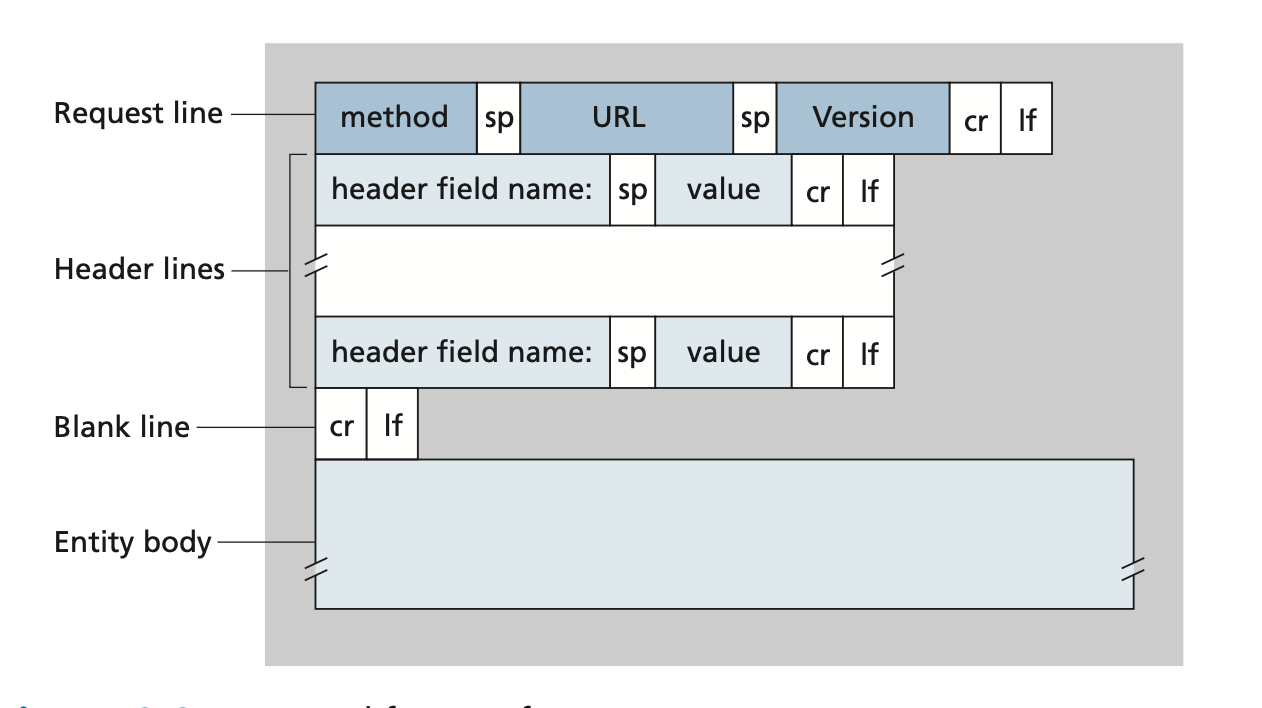
\includegraphics[width=0.8\textwidth]{req.png}
        \caption{General format of an HTTP request message}
        \label{fig:request_message}
    \end{figure}
    \item \textbf{Response Messages:} Response messages are sent by the server to fulfill a client's request for a particular resource. The structure of an HTTP response message typically includes:
    \begin{itemize}
        \item A status line, which includes the HTTP protocol version and a status code indicating the outcome of the request (e.g., 200 for OK, 404 for Not Found, etc.).
        \item Headers, which provide metadata about the response, such as Content-Type specifying the type of data being sent, Content-Length specifying the size of the response body, etc.
        \item An optional message body, which contains the actual data being sent back to the client, such as the HTML content of a web page, image data, or other resources.
    \end{itemize}
     % Insert second image here
    \begin{figure}[h]
        \centering
        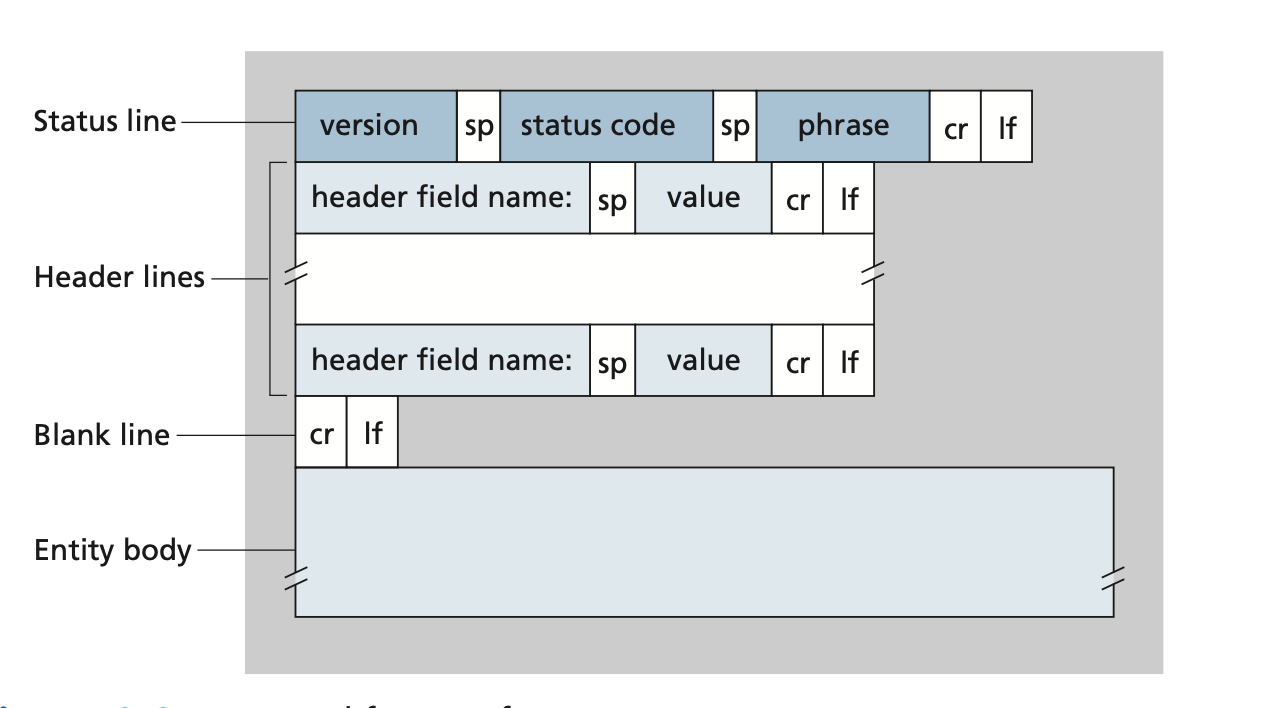
\includegraphics[width=0.8\textwidth]{response.png}
        \caption{General format of an HTTP response message}
        \label{fig:response_message}
    \end{figure}
\end{itemize}
\section{Methodology}
    \subsection{File Transfer via Socket Programming}
        \subsubsection{Server}
Firstly, the server sets up a dedicated directory named "Files" to store the files accessible to clients for download. This directory is prepopulated with sample files for demonstration purposes.

Next, the server establishes socket communication. To handle multiple client connections, the server initiates a new thread for each client using the threading.Thread class. This multithreaded approach allows the server to handle multiple client requests concurrently.

When a client connects to the server, the server sends a list of available files in the "Files" directory to the client.

The server awaits the filename requested by the client. Upon receiving the filename, the server identifies the corresponding file path and begins the file transfer process. If the requested file exists, it is read in binary mode ('rb') and transmitted to the client in chunks of 1024 bytes until the entire file is sent.

Throughout the process, the server provides informative feedback on the status of client connections and file transmissions, printing relevant messages to the server console.

Upon successful completion of file transmission or if the requested file is not found, the server closes the client connection using the close() method.
\subsubsection{Client}

A folder named "Downloads" is defined to store downloaded files. If the folder already exists, it does nothing.

The client initializes a socket. A connection is established with the server using the server's IP address (\texttt{HOST\_IP}) and port number (\texttt{HOST\_PORT}).

After the connection is established, the client receives a list of available files from the server.

The client prompts the user to input the filename they wish to download. The chosen filename is sent to the server using the \texttt{send()} method after encoding it with the specified encoder (\texttt{ENCODER}).

Within the \texttt{receive\_file()} function, the client socket receives data from the server in chunks of 1024 bytes (\texttt{BYTESIZE}). If the received data is not empty, it is written to a file with the specified filename in binary mode (\texttt{'wb'}). This process continues until all data has been received.

After the file transfer process is complete, the client closes the connection with the server using the \texttt{close()} method.


\subsection{File Transfer via HTTP}
    \subsubsection{Server}
The server is initialized with the specified IP address (\texttt{HOST\_IP}) and port number \texttt{HOST\_PORT} using the \texttt{ThreadedTCPServer} class, which extends \newline
\texttt{socketserver.ThreadingMixIn} and \texttt{socketserver.TCPServer}. This allows the server to handle multiple client connections concurrently.
        When a client sends a GET request, the \texttt{do\_GET()} method of the \texttt{FileServer} class is invoked. If the requested file exists and is a regular file, the server sends a 200 OK response with the file attached as an octet-stream for download. If the file does not exist, the server sends a 404 File Not Found error.
        When a client sends a POST request, the \texttt{do\_POST()} method of the \texttt{FileServer} class is invoked. The file data is read from the request body and saved to the server's file system. The server sends a 200 OK response upon successful file upload.

\subsubsection{Client}

The \texttt{download\_file()} function is defined to download files from a specified URL. It takes the URL of the file to download (\texttt{url}) and the path where the file will be saved (\texttt{save\_path}) as input parameters. A GET request is sent to the specified URL using \texttt{requests.get()}. If the response status code is 200 (OK), the file content is written to the specified save path in binary mode ('wb'). Upon successful download, a confirmation message is printed.


The \texttt{upload\_file()} function is defined to upload files to a specified URL. It takes the URL where the file will be uploaded (\texttt{url}) and the path of the file to upload (\texttt{file\_path}) as input parameters. A POST request is sent to the specified URL with the files and headers using \texttt{requests.post()}. Upon successful upload, the server response is printed.


\newpage
\section{Experimental result}
Some Snapshots of the terminal output for each of these tools.
    \subsection{File Transfer via Socket Programming}
    \begin{figure}[h]
        \centering
        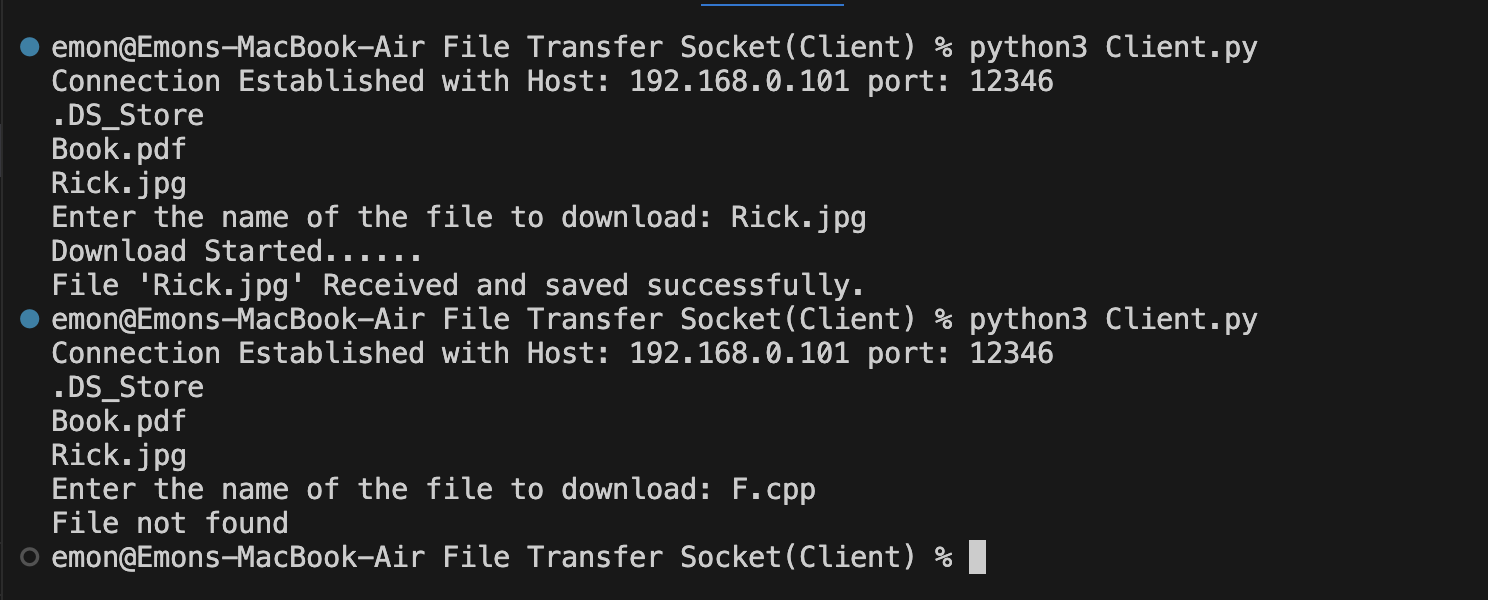
\includegraphics[width=0.8\textwidth]{socket-client.png}
        \caption{Terminal Output for  Client}
        \label{fig:response_message}
    \end{figure}
    \begin{figure}[h]
        \centering
        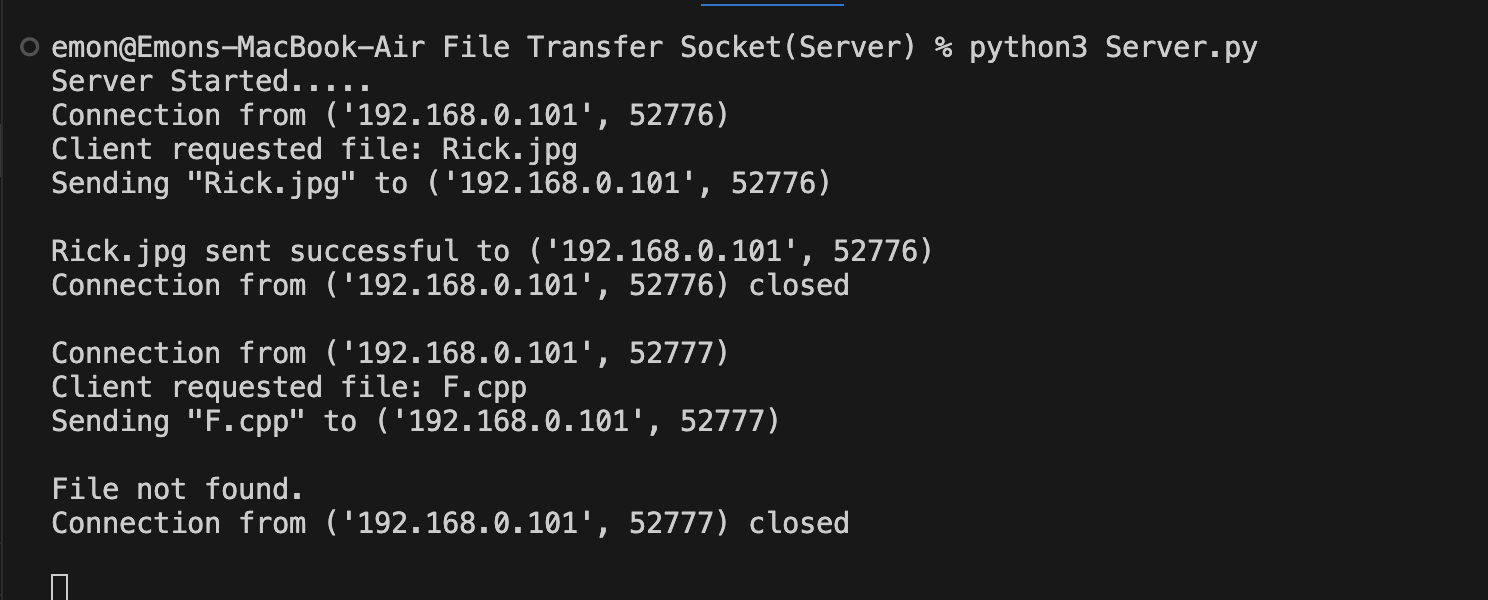
\includegraphics[width=0.8\textwidth]{socket-server.png}
        \caption{Terminal Output for  Server}
        \label{fig:response_message}
    \end{figure}
\newpage
    \subsection{File Transfer via  HTTP}
    \begin{figure}[h]
        \centering
        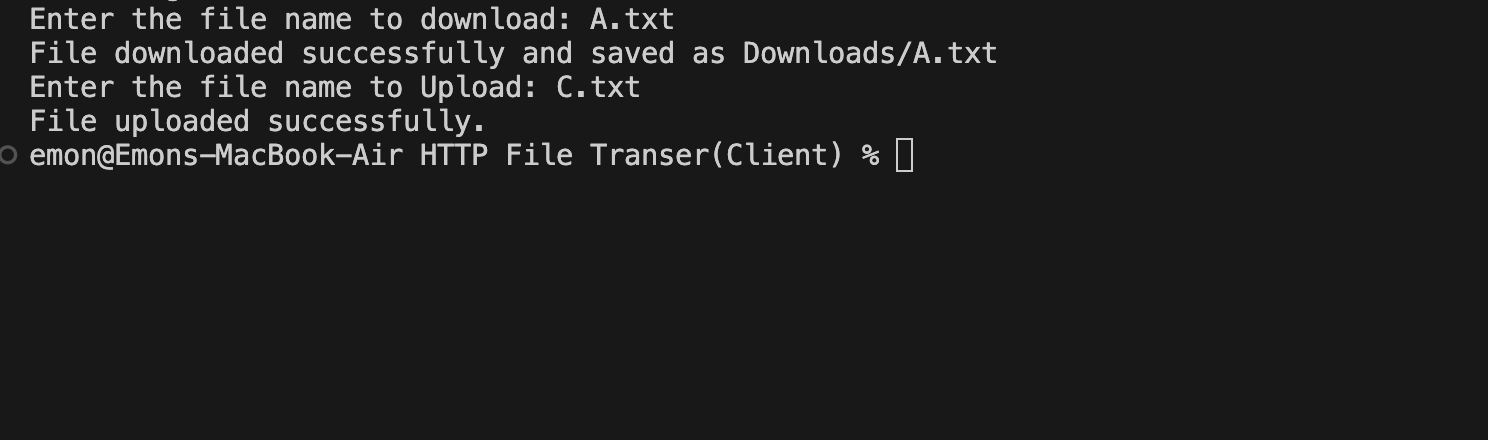
\includegraphics[width=0.8\textwidth]{http-client.png}
        \caption{Terminal Output for  Client}
        \label{fig:response_message}
    \end{figure}
    \begin{figure}[h]
        \centering
        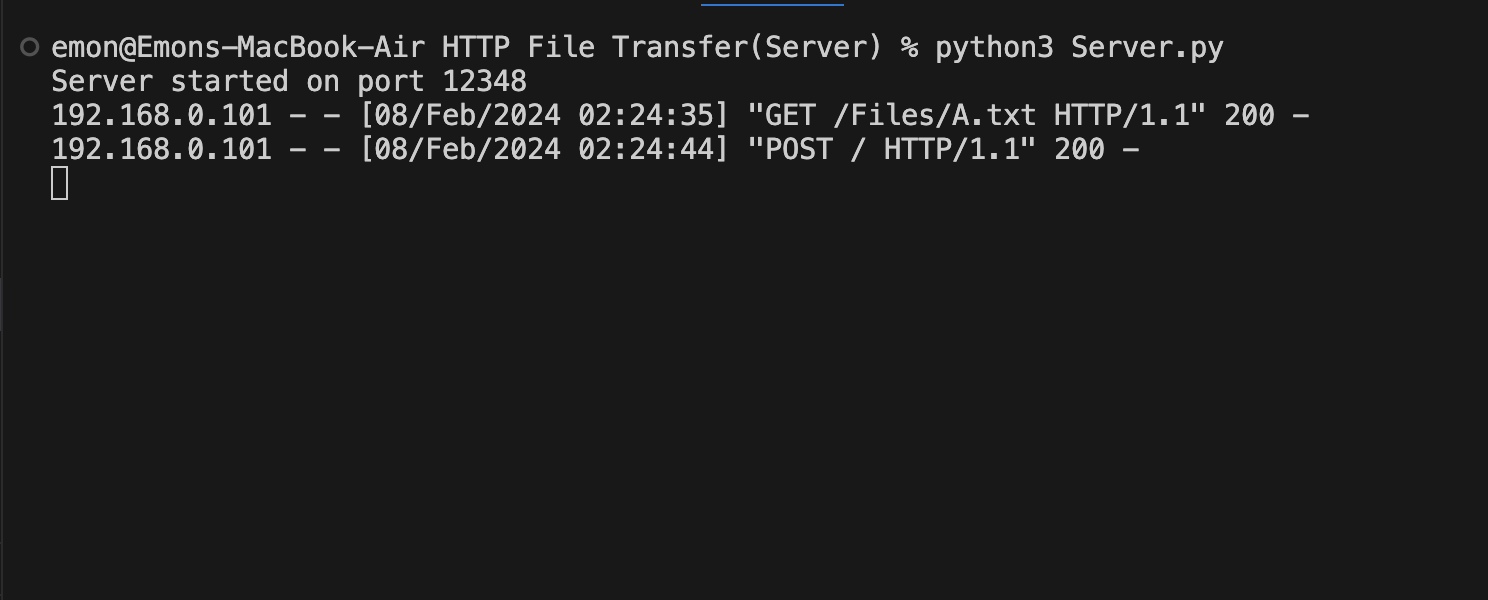
\includegraphics[width=0.8\textwidth]{http-server.png}
        \caption{Terminal Output for  Server}
        \label{fig:response_message}
    \end{figure}

    \begin{figure}[h]
    \centering
    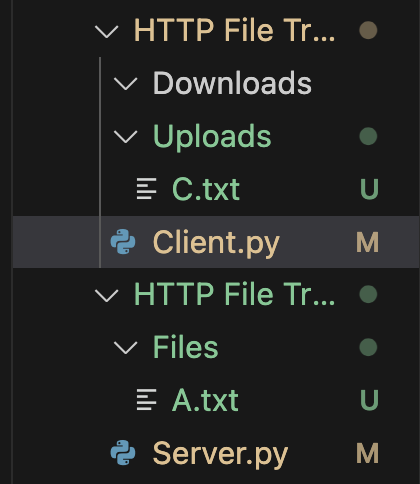
\includegraphics[height=0.6\textwidth]{after.png}
    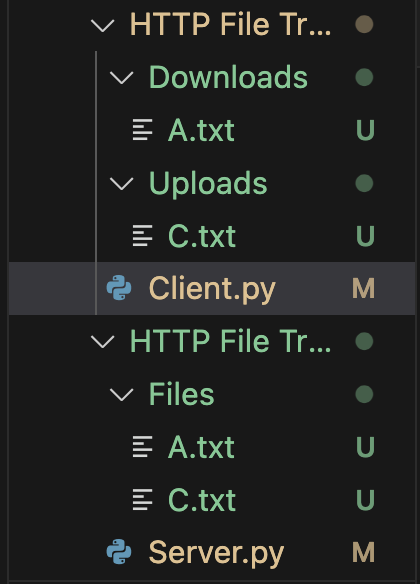
\includegraphics[width=0.43\textwidth]{before.png}
    \caption{Before and After Download and Upload}
    \label{fig:before_after}
\end{figure}

\newpage
\section{Experience}
\begin{enumerate}
    \item We had to look up the server device IP to establish the connection
    \item We established a client-server communication between two different devices using socket programming and sent files via this connection for the first time
    \item We learned the concepts of HTTP GET and POST methods.
    \item Implementation of Multithreaded  System
    \item We learned how errors are handled in a TCP connection
    \item Collaborative Problem-Solving

\end{enumerate}

\newpage
\section*{Appendix}

All the codes are provided in Python programming language

\subsection*{Code for File Transfer via Socket Programming}
\subsubsection*{Server}
\begin{verbatim}
import socket
import threading
import os

#Server Folder
path = 'Files'
files = sorted(os.listdir(path))

def send_file(client_socket, filename, client_address):
    try:
        file_path = os.path.join(path, filename)
        print(f'Sending "{filename}" to {client_address}\n')
        with open(file_path, 'rb') as file:
            data = file.read(1024)
            while data:
                client_socket.send(data)
                data = file.read(1024)
        print(f'{filename} sent successful to {client_address}')
    except FileNotFoundError:
        print("File not found.")

def handle_client(client_socket, client_address):
    print(f"Connection from {client_address}")

    file_list = ':'.join(files)
    client_socket.send(file_list.encode(ENCODER))

    filename = client_socket.recv(BYTESIZE).decode()
    print(f"Client requested file: {filename}")
    send_file(client_socket, filename, client_address)

    client_socket.close()
    print(f"Connection from {client_address} closed\n")


#Connection
HOST_IP = '192.168.0.101'
HOST_PORT = 12346
ENCODER = 'utf-8'
BYTESIZE = 1024

server_socket = socket.socket(socket.AF_INET, socket.SOCK_STREAM)
server_socket.bind((HOST_IP, HOST_PORT))
server_socket.listen(5)
print(f"Server Started.....")

while True:
    client_socket, client_address = server_socket.accept()
    client_handler = threading.Thread(target=handle_client, args=(client_socket, client_address))
    client_handler.start()
\end{verbatim}
\subsubsection*{Client}
\begin{verbatim}
import socket
import os

#Define the Folder Name where the downloaded file will be stored
path = 'Downloads'
try:
    os.makedirs(path)
except FileExistsError:
    pass

def receive_file(server_socket, filename):
    data = server_socket.recv(BYTESIZE)
    if not data.strip():
        print('File not found')
        return
    file_path = os.path.join(path, filename)
    print("Download Started......")
    with open(file_path, 'wb') as file:
        while data:
            file.write(data)
            data = server_socket.recv(BYTESIZE)
    print(f"File '{filename}' Received and saved successfully.")

#Connection
HOST_IP = "192.168.0.101"
HOST_PORT = 12346
ENCODER = 'utf-8'
BYTESIZE = 1024


client_socket = socket.socket(socket.AF_INET, socket.SOCK_STREAM)
client_socket.connect((HOST_IP, HOST_PORT))
print(f"Connection Established with Host: {HOST_IP} port: {HOST_PORT}")

#Receive File List
file_list = client_socket.recv(BYTESIZE).decode(ENCODER).split(":")
for file in file_list:
    if file:
        print(file)

filename = input("Enter the name of the file to download: ")
client_socket.send(filename.encode())
receive_file(client_socket, filename)

client_socket.close()
\end{verbatim}

\subsection*{Code for File Transfer via Socket Programming}
\subsubsection*{Server}
\begin{verbatim}
import http.server
import socketserver
import os
import threading

class FileServer(http.server.SimpleHTTPRequestHandler):
    def do_GET(self):
        try:
            file_path = self.translate_path(self.path)
            
            # Check if the file exists
            if os.path.exists(file_path) and os.path.isfile(file_path):
                # Set headers
                self.send_response(200)
                self.send_header("Content-type", "application/octet-stream")
                self.send_header("Content-Disposition", f"attachment; filename=\"{os.path.basename(file_path)}\"")
                self.end_headers()
                
                with open(file_path, "rb") as file:
                    self.wfile.write(file.read())
            else:
                self.send_error(404, "File Not Found")
        except Exception as e:
            self.send_error(500, f"Internal Server Error: {e}")
            
    def do_POST(self):
        try:
            content_length = int(self.headers['Content-Length'])
            data = self.rfile.read(content_length)
            
            file_name = self.headers['File-Name']
            file_path = os.path.join(os.getcwd(), "Files/" + file_name)
            
            with open(file_path, 'wb') as f:
                f.write(data)
            
            self.send_response(200)
            self.end_headers()
            self.wfile.write(b'File uploaded successfully.')
        except Exception as e:
            self.send_error(500, f"Internal Server Error: {e}")

class ThreadedTCPServer(socketserver.ThreadingMixIn, socketserver.TCPServer):
    pass

# Connection
HOST_IP = '192.168.0.101'
HOST_PORT = 12348

with ThreadedTCPServer((HOST_IP, HOST_PORT), FileServer) as httpd:
    print(f"Server started on port {HOST_PORT}")
    
    try:
        httpd.serve_forever()
    except KeyboardInterrupt:
        print("Server stopped.")

\end{verbatim}
\subsubsection*{Client}
\begin{verbatim}
import requests
import os

def download_file(url, save_path):
    response = requests.get(url)
    if response.status_code == 200:
        with open(save_path, 'wb') as f:
            f.write(response.content)
        print(f"File downloaded successfully and saved as {save_path}")
    else:
        print(f"Failed to download file: {response.status_code}")

def upload_file(url, file_path):
    with open(file_path, 'rb') as f:
        files = {'file': f}
        headers = {'File-Name': os.path.basename(file_path)}
        response = requests.post(url, files=files, headers=headers)
        print(response.text)

#Connection
HOST_IP = '192.168.0.101'
HOST_PORT = 12348
HOST_URL = f'http://{HOST_IP}:{HOST_PORT}/'

# Download
file_name = input("Enter the file name to download: ")
server_file_url = HOST_URL + "Files/" + file_name
save_path = "Downloads/" + file_name
download_file(server_file_url, save_path)

# Upload
file_name = input("Enter the file name to Upload: ")
client_file_url = "Uploads/" + file_name
upload_path = HOST_URL
upload_file(upload_path, client_file_url)
\end{verbatim}


\begin{thebibliography}{1}
    \bibitem{Geeks For Geeks} \url{https://www.geeksforgeeks.org/introducing-threads-socket-programming-java/}
    \bibitem{Geeks For Geeks} \url{https://www.geeksforgeeks.org/transfer-the-file-client-socket-to-server-socket-in-java/}
    \bibitem{Digital Ocean} \url{https://www.digitalocean.com/community/tutorials/java-httpurlconnection-example-java-http-request-get-post}
\end{thebibliography}

\end{document}
